%%%%%%%%%%%%%%%%%%%%%%%%%%%%%%%%%%%%%%%%%%%%%%%%%%%%%%%%%%%%%%%%%%%%%%
% LaTeX Template: Beamer arrows
%
% Source: http://www.texample.net/
% Feel free to distribute this template, but please keep the
% referal to TeXample.net.
% Date: Nov 2006
%
%%%%%%%%%%%%%%%%%%%%%%%%%%%%%%%%%%%%%%%%%%%%%%%%%%%%%%%%%%%%%%%%%%%%%%
% How to use writeLaTeX:4
%
% You edit the source code here on the left, and the preview on the
% right shows you the result within a few seconds.
%
% Bookmark this page and share the URL with your co-authors. They can
% edit at the same time!
%
% You can upload figures, bibliographies, custom classes and
% styles using the files menu.
%
% If you're new to LaTeX, the wikibook is a great place to start:
% http://en.wikibooks.org/wiki/LaTeX
%
%%%%%%%%%%%%%%%%%%%%%%%%%%%%%%%%%%%%%%%%%%%%%%%%%%%%%%%%%%%%%%%%%%%%%%

\documentclass{beamer} %
\usetheme{CambridgeUS}
\usepackage[latin1]{inputenc}
\usefonttheme{professionalfonts}
\usepackage{times}
% \usepackage{tikz}
\usepackage{amsmath}
\usepackage{amssymb}
\usepackage{verbatim}
\usepackage{graphicx}
\usepackage{csquotes}
% \usetikzlibrary{arrows,shapes}

\renewcommand{\vec}[1]{\mathbf{#1}}
\DeclareMathOperator{\sign}{sgn}

\DeclareMathOperator{\EX}{\mathbb{E}}

\author{Jo\"el Faubert}
\title{3D Reconstruction with RGB-D Cameras}

\begin{document}

\begin{comment}
:Title: State of the Art on 3D Reconstruction with RGB-D Cameras
:Tags: Project Proposal for COMP5115
:Use page: 3

\end{comment}

\everymath{\displaystyle}

\begin{frame}
%\frametitle{Title}

\begin{center}
{\Large Zollh\"ofer, Michael et al.

STAR: Reconstruction with RGB-D}

COMP5115 - Fall 2019
\end{center}
\end{frame}

\begin{frame}
\frametitle{Outline}

\begin{itemize}
\item Introduction
\item Static Scene Reconstruction
\item Capturing Dynamic Scenes
\item Color and Appearance
\end{itemize}

\end{frame}


\begin{frame}
\frametitle{Method -- Overview}

Dense SLAM with Active Depth Sensing is an online scene reconstruction system
composed of 4 steps:

\begin{enumerate}
  \item Surface Measurement: pre-processing, generate vertex data \& normals
  \item Surface Reconstruction Update: use pose estimation to integrate new surface measurements into
  global scene model (TSDF).
  \item Surface Prediction: generate dense surface prediction to align new depth maps.
  \item Sensor Pose Estimation: multi-scale ICP align between predicted surface and current measurement.
\end{enumerate}
\end{frame}

\begin{frame}
\frametitle{Method -- Overview 2}

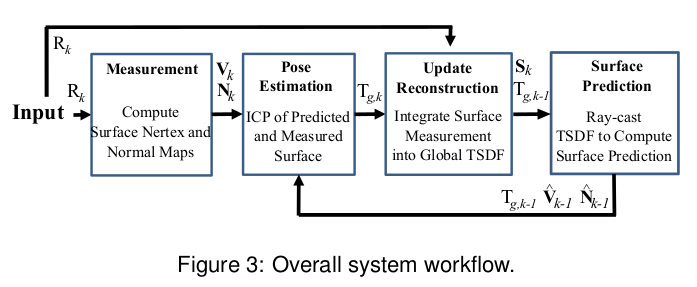
\includegraphics[scale=0.45]{img/method_diagram.png}
\end{frame}


\begin{frame}
\frametitle{Method -- Math Preliminaries}
6 degree of freedom pose estimation representated as matrix

\[ T_{g,k} = \begin{bmatrix} R_{g,k} & t_{g,k} \\ \mathbf{0}^T & 1 \end{bmatrix} \]

(an element Special Euclidean group -- translations \& rotations but not reflections)

It maps camera coordinate frame at time $k$ into global frame $g$.
Point $p_k \in \mathbb{R}^3$ in camera space is transferred
to global coordinate space via

\[ p_g = T_{g,k} p_k \]


\end{frame}


\begin{frame}
\frametitle{Method -- Math Preliminaries 2}

Three different reference frames for points: camera frustum, projective space (camera pixels) and
global model.

Camera matrix $K$ transforms points on the depth surface into image pixels.
and $\pi (p)$ performs perspective projection (dehomogenization) to obtain
camera pixel $q \in \mathbb{R}^2 = (x/z, y/z)^T$

\end{frame}


\begin{frame}
\frametitle{Method -- Surface Measurement}

Raw depth map $R_k$ at time $k$ gives calibrated depth $R_k(u) \in \mathbb{R}$ at
each pixel $u = (u,v)^T$ for $u \in \mathcal{U} \subset \mathbb{R}^2$ (camera pixel space).

\[ \vec{p_k} = R_k(\vec{u})K^{-1}\dot{\vec{u}} \]

$p_k$ is a metric point measurement in sensor frame $k$.

\end{frame}

\begin{frame}
\frametitle{Method -- Surface Measurement 2}

Apply \textit{bilateral filter} to raw depth map to smooth noise.

\[ D_k(\vec{u}) = \frac{1}{W_p} \sum_{\vec{q} \in \mathcal{U}} \mathcal{N}_{\sigma_s}(||\vec{u}-\vec{q}||_2) \mathcal{N}_{\sigma_r}(||R_k(\vec{u}) - R_k(\vec{q})||_2)R_k(\vec{q}) \]

Where $W_p$ is a normalizing constant (two Gaussians) and $\sigma_r$ and $\sigma_s$ are
parameters.

\end{frame}

\begin{frame}
\frametitle{Method -- Surface Measurement 3}
{\large Vertex \& Normal Maps}

Create vertex map $V_k$ by projecting filtered depth values back into sensor's frame of reference:

\[ V_k{\vec{u}} = D_k(\vec{u})K^{-1}\dot{\vec{u}} \]

Depth sensor frames are measurements on a regular grid so can approximate normals using
neighbours easily:

\[ N_k(\vec{u}) = v\left[(V_k(u+1, v) - V_k(u,v)) \times V_k(u, v+1) - V_k(u,v)\right] \]

where $v[x] = \hat{x}$
\end{frame}

\begin{frame}
\frametitle{Method -- Surface Measurement 4}
{\large Validity Mask}

Also need to keep track of sensor failures. Use \textit{validity mask}

\[ M_k(\vec{u}) = \begin{cases} 1 & \text{depth measure transforms to valid vertex?} \\
  0 & \text{otherwise} \end{cases} \]

Finally, create ``multi-scale representation of surface measurement in form of a vertex and
normal pyramid.''

Depth \textit{pyramid} is a sequence $D^{l \in [1 \dots L ]}$ created by stacking
depth map with sub-sample layers created by block-averaging (convolution?).
\end{frame}

\begin{frame}
\frametitle{Method -- Surface Measurement 5}

Authors use $L=3$ and are careful to ``discard depth values more than $3\sigma_r$
of the central pixel to avoid smoothing over depth boundaries''.

Vertex and normal pyramids are then $V^{l \in [1 \dots L]}$ and $N^{l \in [1 \dots L ]}$
computed using corresponding depth pyramid layer.

\[V_g^k(\vec{u}) = T_{g,k}\dot{V_k(\vec{u})} \]
\[N_g^k(\vec{u}) = R_{g,k}N_k(\vec{u}) \]
\end{frame}


\begin{frame}
\frametitle{Method -- Mapping as Surface Reconstruction}
{\Large Global \& Current TSDF}

Function $S_k(\vec{p})$ is a fusion of TSDFs estimated
 from frames $1 \dots k$ (where $p \in \mathbb{R}^3$ a global frame point in 3D volume).

\[ S_k(\vec{p}) \mapsto [F_k(p), W_k(p)] \]

Assuming sensor error $\mu$, dense surface measurement provides two constraints
\[ r \overset{?}{<} (\lambda R_k(\vec{u}) - \mu) \]
where $\lambda = || K^{-1}\dot{u}||$.

If less, detected free space. No surface information is obtained in reconstruction volume.
Discard these values.
\end{frame}

\begin{frame}
\frametitle{Method -- Mapping as Surface Reconstruction}

For raw map $R_k$ with known pose $T_{g,k}$, its global frame projective
TSDF is $[F_{R_k}, W_{R_k}]$ at a point $\vec{p}$ in the global frame is computed as

\[ F_{R_k} = \Psi\left( \lambda^{-1} (||\vec{t_{g,k}} - \vec{p}||_2 - R_k(\vec{x}))\right) \]
\[ \lambda = ||K^{-1}\dot{x}||_2 \]
\[ \vec{x} = \left\lfloor \pi (KT^{-1}_{g,k}\vec{p})\right\rfloor \]
\[ \Psi(\eta) = \begin{cases}
\min(1, \frac{\eta}{\mu}) \sign(\eta) & \eta \geq - \mu \\
\text{null} & \text{otherwise}
\end{cases} \]

And $W_{R_k} \propto \cos (\theta) / R_k(x)$ where $\theta$ angle between
associated pixel ray direction and surface normal in local frame.

\end{frame}


\input{results.tex}

\begin{frame}[allowframebreaks]
  \frametitle<presentation>{References}
  \begin{thebibliography}{1}
  \beamertemplatearticlebibitems
  \bibitem{zollhofer2018state}
    Zollh{\"o}fer, Michael et al. (2018)
    \newblock State of the Art on 3D Reconstruction with RGB-D Cameras
    \newblock Computer Graphics Forum
  \bibitem{pagliari2014kinect}
    Pagliari, Diana and Menna, Fabio and Roncella, R and Remondino, Fabio and Pinto, Livio (2011)
    \newblock Kinect Fusion improvement using depth camera calibration
    \newblock Photogrammetry, Remote Sensing and Spatial Information Sciences
  \end{thebibliography}
\end{frame}


\end{document}
